\documentclass[]{interact}

%\usepackage[caption=false]{subfig}% Support for small, `sub' figures and tables
%\usepackage[nolists,tablesfirst]{endfloat}% To `separate' figures and tables from text if required
%\usepackage[doublespacing]{setspace}% To produce a `double spaced' document if required
%\setlength\parindent{24pt}% To increase paragraph indentation when line spacing is doubled
%\setlength\bibindent{2em}% To increase hanging indent in bibliography when line spacing is doubled

\usepackage[numbers,sort&compress]{natbib}% Citation support using natbib.sty
\bibpunct[, ]{[}{]}{,}{n}{,}{,}% Citation support using natbib.sty
\renewcommand\bibfont{\fontsize{10}{12}\selectfont}% Bibliography support using natbib.sty

\usepackage{amsmath}
\usepackage{stmaryrd}  % \llbracket, \rrbracket

\usepackage{algorithm}
\usepackage{algpseudocode}
\usepackage[T1]{fontenc}
\usepackage{pgfplots}
\usetikzlibrary{arrows}
\pgfplotsset{compat=1.16}
\usepackage{caption}
\usepackage{subcaption}
%\usepackage{minted}

\usepackage[hidelinks]{hyperref}

\theoremstyle{plain}% Theorem-like structures provided by amsthm.sty
\newtheorem{theorem}{Theorem}[section]
\newtheorem{lemma}[theorem]{Lemma}

\newtheorem{corollary}[theorem]{Corollary}
\newtheorem{proposition}[theorem]{Proposition}

\theoremstyle{definition}
\newtheorem{definition}[theorem]{Definition}
\newtheorem{example}[theorem]{Example}

\theoremstyle{remark}
\newtheorem{remark}{Remark}
\newtheorem{notation}{Notation}

\newcommand{\RR}{\mathbb{R}}

\newcommand{\eps}{\epsilon}
\newcommand{\grad}{\nabla}
\newcommand{\Div}{\nabla\cdot}

\newcommand{\bn}{\mathbf{n}}

\newcommand{\bX}{\mathbf{X}}

\newcommand{\cK}{\mathcal{K}}
\newcommand{\cT}{\mathcal{T}}
\newcommand{\cX}{\mathcal{X}}

\begin{document}

%\articletype{ARTICLE TEMPLATE}% Specify the article type or omit as appropriate

\title{Pragmatic adaptive mesh refinement for obstacle problems}

\author{
\name{G.~Stefano Fochesatto\thanks{CONTACT G.~Stefano Fochesatto Email: gsfochesatto@alaska.edu} and Ed Bueler}
\affil{Dept.~of Mathematics and Statistics, University of Alaska Fairbanks, USA}
}

\maketitle

\begin{abstract}
Free-boundary problems posed as variational inequalities, for example obstacle problems, appear in many scientific and engineering applications.  In the finite element solution of these problems, the geometrical error in locating the unknown free boundary, equivalently in locating the active and inactive sets, often dominates the overall numerical error.  In this paper we propose, and implement using the Firedrake finite element library, parallel adaptive mesh refinement strategies which enhance mesh resolution around the free boundary.  These methods mark elements for refinement based on a computed solution.  We consider three methods: (i) an unstructured dilation operator which computes discrete adjacency to the computed free-boundary; (ii) a variable-coefficient diffusion method which thresholds a diffused indicator function for the computed active set; and (iii) a metric-based method which averages an anisotropic, Hessian-derived Riemannian metric with an isotropic metric computed from the same diffused active set indicator.  These methods, along with hybrid strategies adding classical \emph{a posteriori} error estimators in the computed inactive sets, are evaluated by norm error relative to mesh complexity and run-time, and by geometrical error in set localization using Jaccard and Hausdorff distances.  Applications include classical Laplacian obstacle problems and a shallow ice flow problem for predicting the glaciated region in a mountain range.
\end{abstract}

%\begin{keywords}
%FIXME
%\end{keywords}


\section{Introduction} \label{sec:intro}

The classical Laplacian obstacle problem \cite{KinderlehrerStampacchia1980} finds the equilibrium position (vertical displacement) $u$ of an elastic membrane over some domain $\Omega \subset \RR^d$.  The membrane is constrained to be above a given obstacle $\psi$, while also attached with displacement $g$ at the fixed boundary $\partial\Omega$, and subjected to some applied force $f$.  The strong formulation of this problem is a complementarity problem satisfied almost everywhere in $\Omega$:
\begin{subequations} \label{eq:classical:ncp}
\begin{align}
  -\nabla^2 u - f \geq 0 \label{eq:classical:ncp:a} \\
  u - \psi \geq 0\\
  (-\nabla^2u - f)(u - \psi) = 0 \label{eq:classical:ncp:c}
\end{align}
\end{subequations}
From a solution to \eqref{eq:classical:ncp} we may identify the inactive and active sets,
\begin{equation}
  I_u = \{x \in \Omega \,:\, u(x) > \psi(x)\}, \quad A_u = \Omega \setminus I_u, \label{eq:classical:sets}
\end{equation}
and the free boundary
\begin{equation}
\Gamma_u = \Omega \cap \partial I_u, \label{eq:classical:freeboundary}
\end{equation}
which is where $I_u$ meets $A_u$ within $\Omega$.  Note that $u$ solves the Poisson equation $-\nabla^2u = f$ on $I_u$; this gives the interior condition of the free-boundary problem.  Both Dirichlet ($u=\psi$) and Neumann ($\grad u = \grad \psi$) conditions apply along the unknown set $\Gamma_u$, while only fixed Dirichlet conditions ($u=g$) hold along $\partial\Omega$.

For the example shown in Figure \ref{fig:ball}, $A_u$ is a disc and $\Gamma_u=\partial A_u$ is a circle.

\begin{figure}[H]
\centering
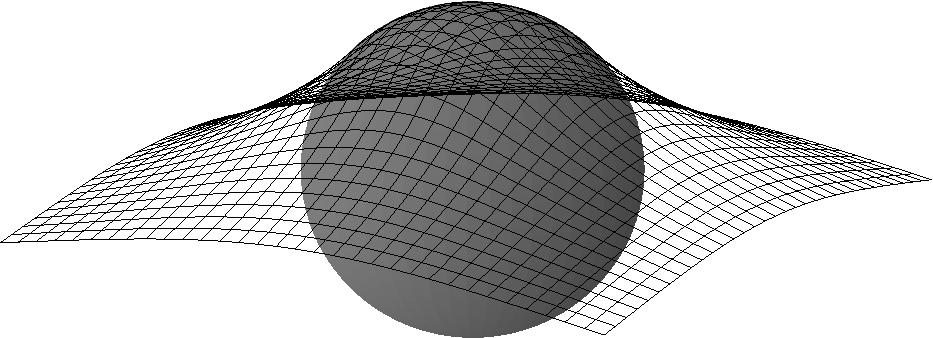
\includegraphics[width=0.7\textwidth]{static/obstacle65.pdf}
\caption{A classical obstacle problem with a hemispherical obstacle.}
\label{fig:ball}
\end{figure}

As is well-known, problem \eqref{eq:classical:ncp} has a weak formulation which is a variational inequality (VI) over a Sobolev space.  Let $\cX=H^1(\Omega)$ \cite{ElmanSilvesterWathen2014} and suppose $\psi \in \cX \cap C(\bar\Omega)$.  (In a faithful visualization, Figure \ref{fig:ball} would show $\psi$ as most of the upper hemisphere of the ball, extended continuously to the fixed boundary.)  Let $g:\partial \Omega\to \RR$ be continuous, with $\psi|_{\partial \Omega} \le g$.  Let
\begin{equation} \label{eq:classical:admissible}
\cK = \{u \in \cX \,:\, u \ge \psi \text{ and } u|_{\partial \Omega} = g\}
\end{equation}
be the admissible subset for solutions, closed and convex in $\cX$.  For $f\in L^2(\Omega)$, the VI formulation of the obstacle problem \cite{KinderlehrerStampacchia1980} finds $u\in \cK$ so that
\begin{equation} \label{eq:classical:vi}
\int_\Omega \nabla u \cdot \nabla(v - u) \ge \int_\Omega f(v - u) \quad \text{ for all } v \in \cK.
\end{equation}

Section \ref{sec:vifem} will recall some theory of such VIs, and their finite element (FE) approximation, but generalized from elliptic bilinear forms, as in \eqref{eq:classical:vi}, to coercive nonlinear operators over Banach spaces.  A conforming FE approximation of such a VI uses the same weak form, but now over a discrete space constructed on a mesh $\cT_h$.  Similarly to Cea's lemma for PDEs \cite{ElmanSilvesterWathen2014}, the norm errors $\|u-u_h\|$ can be bounded \emph{a priori} by extending the Falk \cite{Falk1974} technique to nonlinear operators (Theorem \ref{thm:genfalk}).  Then these norm errors are controlled by the approximation properties of the FE space, but here with additional VI-specific concerns regarding admissibility and the construction of the FE obstacle.

Adaptive mesh refinement (AMR) uses \emph{a posteriori} information from a coarser-mesh calculation to strategically add elements to a mesh, to reduce numerical error.  For VI problems the geometrical (mesh) error in locating the free-boundary $\Gamma_u$ can, by itself, strongly impact the behaviour of the numerical error $\|u-u_h\|$.  This fact, acknowledged in the FE literature for VIs \cite{Suttmeier2008}, is clearly seen in the following 1D example.

\begin{example} \label{example:oned} Suppose $\Omega = (-1,1)$, $\psi(x)=0.5 - x^2$, $f=0$, and $g=0$.  The exact solution $u$ of \eqref{eq:classical:vi} for this data is easily calculated.  Free boundaries are at $x_*=\pm(1-2^{-1/2})$ (Figure \ref{fig:parabola}).  For an FE approximation using piecewise-linear elements and a uniform mesh, let $\Delta_h$ be the minimum distance between a node and $x_*$.  Noting that $x_*$ are irrational, under uniform refinements $\Delta_h = O(h)$ is an irregular function of $h$.  Figure \ref{fig:parabola} (right) compares $H^1$ and $L^2$ norm errors to $\Delta_h$.  The erratic behavior of the norm errors closely follows the purely-geometrical free-boundary location error $\Delta_h$. \end{example}

\begin{figure}[ht]
\mbox{
\begin{minipage}[t]{0.45\textwidth}
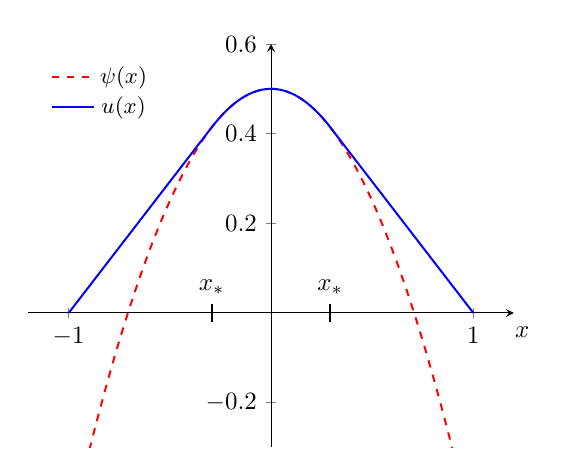
\begin{tikzpicture}[scale=0.9]
    \begin{axis}[
      axis lines = middle,
      xlabel = {$x$},
      xlabel style = {at={(1.05, 0.25)}},  % relative to whole figure box [0,1]x[0,1]
      domain = -1:1,
      samples = 100,
      xmin = -1.2,
      xmax = 1.2,
      ymin = -0.3,
      ymax = 0.6,
      xtick = {-1,1},
      legend pos = north west,
      legend style = {draw=none, font=\small}
    ]
      % Parameters
      \def\b{(2-sqrt(2))/2}
      \def\a{-\b}
      % Plot the obstacle function psi(x)
      \addplot[
        thick,
        red,
        dashed
      ] {0.5 - x^2};
      \addlegendentry{$\psi(x)$}
  
      % Plot u(x) in three pieces
      \addplot[
        thick,
        blue,
        domain=-1:\a
      ] {((.5 - \a*\a)/(\a + 1))*(x + 1)};
      \addplot[
        thick,
        blue,
        domain=\a:\b
      ] {0.5 - x^2};
      \addplot[
        thick,
        blue,
        domain=\b:1
      ] {-((.5 - \b*\b)/(1 - \b))*(x - 1)};
      \addlegendentry{$u(x)$}

      % indicate free boundary locations
      \addplot[black, thick, draw] coordinates {(\a,-0.02) (\a,0.02)} node[above] (A) {$x_*$};
      \addplot[black, thick, draw] coordinates {(\b,-0.02) (\b,0.02)} node[above] (B) {$x_*$};
    \end{axis}
  \end{tikzpicture}
  
\end{minipage}
\quad
\begin{minipage}[t]{0.55\textwidth}
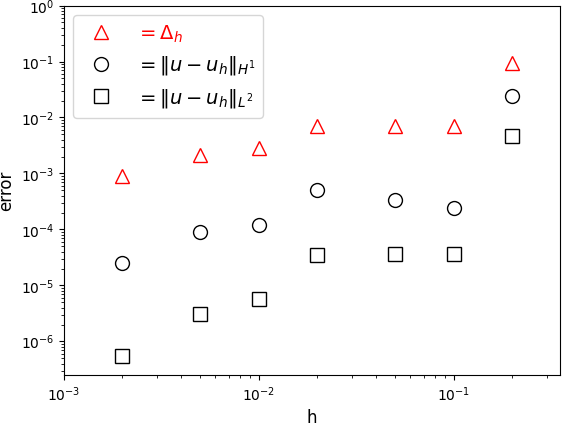
\includegraphics[width=0.9\textwidth]{static/VIConvergence.png}
% FIXME regenerate with labels ||u-u_h||_{H^1} = O(h^1.09), ||u-u_h||_{L^2} = O(h^1.57), \Delta_h
\end{minipage}
}
\caption{A one-dimensional obstacle problem (left), for which the geometrical free-boundary location error $\Delta_h$ predicts norm error $\|u-u_h\|$ behavior (right).}
\label{fig:parabola}
\end{figure}

A small modification of Example \ref{example:oned} illustrates another aspect of obstacle problems, namely that the sets $A_u,I_u,\Gamma_u$ are \emph{not} continuous functions of the data in general.

\begin{example} \label{example:notcontinuous} Suppose we change Example \ref{example:oned} by setting $g=-0.5$, so that $g=\psi$ on $\partial\Omega$.  For $\eps\in\RR$ we define a new source term $f_\eps(x)=2+\eps$.  An easy calculation shows that for $\eps\le 0$ the solution is $u_\eps=\psi$, thus $A_{u_\eps}=\Omega$ and $I_{u_\eps}=\emptyset$.  However, for $\eps>0$, so that $f_\eps$ represents sufficient upward force on the membrane to lift it off the obstacle, we find the solution satisfies $u_\eps(x)=\psi(x) + 0.5 \eps (1-x^2) > \psi(x)$ for all $x\in\Omega$.  Thus $A_{u_\eps}=\emptyset$ and $I_{u_\eps}=\Omega$ for $\eps>0$, so these sets are discontinuous functions at $\eps=0$. \end{example}

By definition, the $\eps=0$ case of Example \ref{example:notcontinuous} is \emph{degenerate} \cite{KinderlehrerStampacchia1980}, that is, the unconstrained solution happens to match the obstacle.  This example shows that any predictable convergence results for FE approximations of the solution-dependent sets \eqref{eq:classical:sets}, \eqref{eq:classical:freeboundary} will depend upon nondegeneracy assumptions of some kind.

The effectiveness of AMR strategies for VI problems will depend upon the measure (area or volume) of the active and inactive sets.  Note that for obstacle-type problems, those elements which have been correctly identified as interior to the active set generally require no further computation or refinement.  (If a solution is desired at high resolution within the active set, this can be computed \emph{a posteriori} by arbitrary interpolation of the obstacle, because $\psi$ has already been provided in the data of the problem.)

\begin{example} \label{example:activesets} In Section \ref{sec:results} we will measure convergence rates for three classical obstacle problem examples in 2D.  Figure \ref{fig:activesizes} shows high-resolution active sets for these examples.  For the large active set case at right, we will see that most of the performance benefit of our preferred AMR techniques, relative to uniform refinement, comes from avoiding refinement in the active set.  This benefit also dominates performance for our glaciation application in Section \ref{sec:app}. \end{example}

\begin{figure}[ht]
\noindent \hspace{-1mm} \mbox{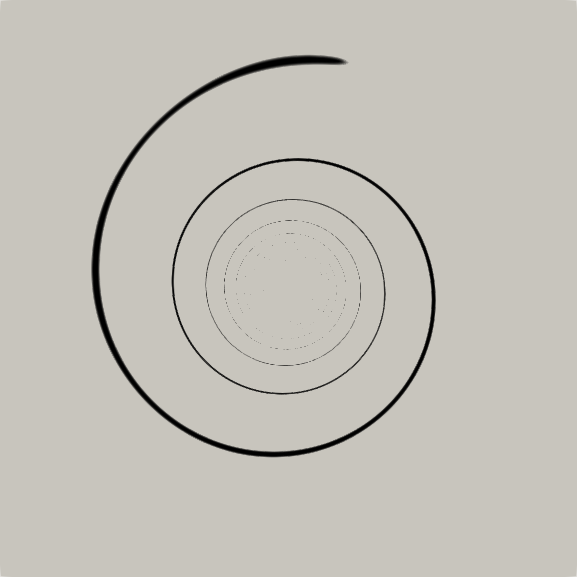
\includegraphics[width=0.32\textwidth]{static/spiral.png} \,
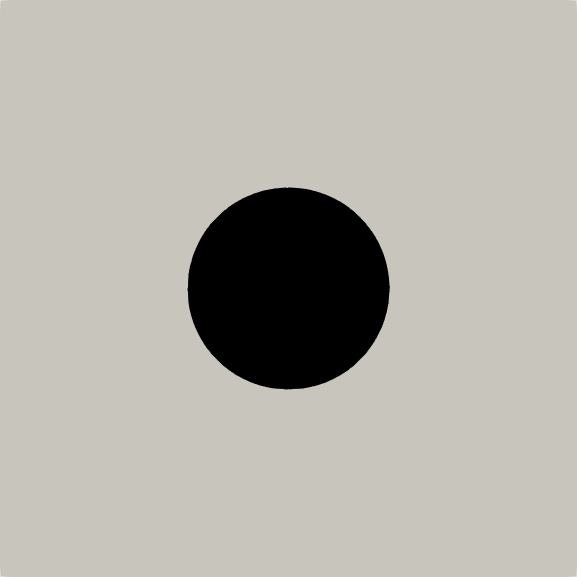
\includegraphics[width=0.32\textwidth]{static/sphere.png} \,
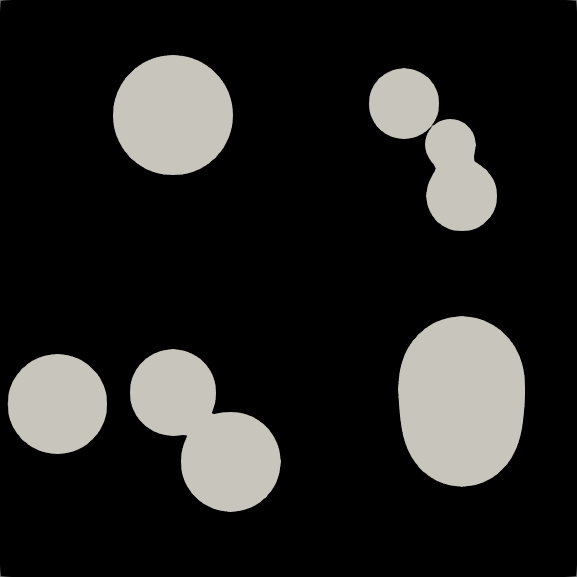
\includegraphics[width=0.32\textwidth]{static/blisters.png}}
\caption{The area (measure) of the active set (black) of the solution of a classical obstacle problem can vary from small to large (left to right); the middle subfigure is for the same problem as Figure \ref{fig:ball}.}
\label{fig:activesizes}
\end{figure}

In this work we consider only meshs of triangles or tetrahedra, and $P_1$ elements (Section \ref{sec:results}), and only $h$-refinement is addressed.  VIs can be solved using $p$-refinement and higher-order elements, but only if nontrivial monotonicity modifications are made \cite{KeithSurowiec2024}, which is not attempted here.  Also, note that the classical obstacle problem in VI form \eqref{eq:classical:vi} is equivalent to constrained minimization of a scalar objective \cite{KinderlehrerStampacchia1980}.  However, the analysis of FE errors for VI problems presented in Section \ref{sec:vifem} does not require such an objective, nor do our AMR strategies exploit one if available, and indeed no objective exists for the application in Section \ref{sec:app}.

Three AMR methods for VIs are described in Section \ref{sec:viamr}.  Our implementations use the Firedrake finite element library \cite{Rathgeberetal2016} and produce conforming meshes with no hanging nodes.  The first two methods are of tag-and-refine type, only differing by which elements are tagged.  For these methods skeleton-based refinement \cite{PlazaCarey2000} is applied after tagging, as implemented within PETSc's DMPlex component \cite{petsc-user-ref} or by calls to the Netgen library \cite{Betteridgeetal2024}.  The third method is goal-oriented and metric-based \cite{Wallworketal2020}.  While full details are given in Section \ref{sec:viamr}, the following is a high-level summary:

\renewcommand{\labelenumi}{(\roman{enumi})}
\begin{enumerate}
\item The unstructured dilation operator (UDO) method discretely identifies elements adjacent to the computed free boundary, employing a graph-based approach to tag neighboring elements for refinement.  It generalizes the bit-map image processing operation of dilation \cite{Pratt1991} to unstructured meshes.
\item The variable-coefficient diffusion (VCD) method starts from a node-wise indicator function for the current computed active set.  This indicator becomes the initial iterate in a single step of a time-dependent heat equation problem.  Solving this problem smooths the indicator about the free boundary.  The smoothed indicator is then averaged over each element and thresholded for element tagging.
\item The averaged-metric (AVM) method computes an intermediate representation of the size, shape, and orientation of the new mesh, namely a tensor-valued Riemannian metric \cite{Alauzet2010}.  The metric averages the Hessian of the computed solution with an isotropic metric generated from the same diffused active set indicator as in VCD.  Then the mesh is actually refined using the MMG mesh library \cite{DapognyDobrzynskiFrey2014}.  This permits controlled anisotropy \cite{Wallworketal2020} to reduce inactive set solution norm error, while approximately maintaining mesh complexity.
\end{enumerate}

The numerical results in Sections \ref{sec:results} and \ref{sec:app}, from applying these three strategies, will justify our somewhat-heuristic approach to AMR for VIs.  Because the convergence of VI problems is dominated by the error in approximating the free boundary, an AMR scheme that quickly concentrates effort around an accurately-computed free boundary, and which applies PDE-type error estimators in the inactive set (Section \ref{sec:vifem}), will enhance norm and geometrical convergence while reducing unnecessary computation.

AMR for VI problems has been explored in the literature.  The first published analysis may be \cite{AinsworthOdenLee1993}, giving an error bound for the classical obstacle problem in terms of local functionals associated with each element.  The monograph by Suttmeier \cite{Suttmeier2008} covers a broader class of problems, including elasticity.  The constructable error estimators in these works, even for the classical obstacle problem, require heuristic assumptions which may not hold in general.  (See inequality (42) in \cite{AinsworthOdenLee1993}, and the approximation ``$(u-\psi)\lambda_h\approx 0$'' in \cite{Suttmeier2008}.)  To our knowledge these approaches are not found in publicly-available implementations, nor are they as efficient as the best of our strategies, when computing high-resolution approximations to free boundaries.

Our focus in this paper is on AMR performance, but not solver performance.  Since the constraint $u \geq \psi$ makes VI problems nonlinear, even if the operator is linear, an iterative solver is required.  We use a VI-adapted, reduced-space Newton method with line search \cite{BensonMunson2006}, implemented in PETSc \cite{petsc-user-ref}.  Such a numerical method cannot converge quadratically until the active and inactive sets stabilize on the given mesh, equivalently once the discrete free boundary is identified.  Then convergence occurs in one additional iteration when the operator is linear,  otherwise in a few iterations for well-behaved operators.  Such a reduced-space Newton solver can only adjust the approximated free boundary by one-cell per iteration \citep{GraeserKornhuber2009}, and thus overall convergence becomes proportional to the number of grid spaces between the initial-iterate free boundary and the solution free boundary \citep{Bueler2021}.

Such poor geometrical VI solver performance could be substantially improved by combining the AMR meshing strategies here with a multilevel solver like that in \cite{BuelerFarrell2024}, which uses coarse corrections to generate large geometrical corrections in the free boundary.  This path, promising highly-scalable solutions of obstacle problems, is for future research.

To conclude this introduction, there are two overall goals for this paper:
\renewcommand{\labelenumi}{\arabic{enumi}.}
\begin{enumerate}
\item We demonstrate significant, practical improvements in error norm convergence for obstacle problems, arising from the application of AMR, relative to high-resolution uniform-refinement approaches such as \cite{BuelerFarrell2024}.  This is measured by error norm (or free-boundary localization error) per mesh degree of freedom.
\item We provide a parallel, well-documented, and easy-to-use implementation, hosted at \url{https://github.com/StefanoFochesatto/VI-AMR}, within a widely-distributed FE library framework, namely Firedrake \cite{Langeetal2016}.
\end{enumerate}

The remaining material is organized as follows.  Table \ref{tab:abbrev} gives the few abbreviations used herein.  Section \ref{sec:vifem} provides \emph{a priori} norm bounds for FE methods applied to VI problems, and \emph{a posteriori} error estimators which can be applied to the PDE solved in the inactive set.  Section \ref{sec:viamr} describes the three AMR algorithms in more detail.  Sections \ref{sec:results}--\ref{sec:conclusion} compare and discuss the performance of these algorithms on model problems and on a realistic application to glaciers.

\begin{table}[ht]
\centering
\begin{tabular}{ll}
AMR       & adaptive mesh refinement \\
AVM$^*$   & averaged-metric \\
BR        & Babu\v{s}ka--Rheinboldt, an error estimator \\
%DWR       & dual-weighted residual error estimate \\
FE        & finite element \\
PDE       & partial differential equation \\
UDO$^*$   & unstructured dilation operator \\
VCD$^*$   & variable-coefficient diffusion \\
VI        & variational inequality
\end{tabular}

\caption{Abbreviations used in this paper.  Stars indicate the new AMR methods.}
\label{tab:abbrev}
\end{table}


\section{Variational inequalities and their finite element approximation} \label{sec:vifem}

We start this Section with the VI formulation of unilateral obstacle problems in Banach spaces.  Under a hypothesis of coercivity we have continuum well-posedness, even for nonlinear operators.  Then we consider the meaning of ``conforming FE methods'' for such problems, and prove an \emph{a priori} bound on FE norm error which extends the Falk \cite{Falk1974} technique for VIs, itself generalizing Cea's lemma \cite{ElmanSilvesterWathen2014} for PDE problems.  This bound can illuminate why targeted mesh refinement around the computed free boundary will generate improved solutions.  Then we provide a classical \emph{a posteriori} error estimator for PDEs, considering its application in the computed inactive set.  We also aim to correct some misperceptions in the FE literature for VI problems.

For a bounded, open domain $\Omega \subset \RR^d$, $d=2,3$, with Lipschitz boundary \cite{Ciarlet2002}.  In fact, for simplicity we will assume that $\Omega$ is polygonal or polyhedral.  Let $\cX = W^{1,p}(\Omega)$, $p>1$, be the Sobolev space of measurable functions with $p$th-integrable gradients \cite{Evans2010}.  We will assume continuous problem data, allowing well-defined point values, so suppose $\psi \in \cX \cap C(\bar\Omega)$ and $g\in C(\partial \Omega)$ satisfy $g \ge \psi|_{\partial\Omega}$.  As with the classical obstacle problem \eqref{eq:classical:admissible}, define the admissible subset
\begin{equation} \label{eq:admissible}
\cK = \{v \in \cX \,:\, v \ge \psi \text{ and } v|_{\partial \Omega} = g\}
\end{equation}
Note that $\cK\subset \cX$ is closed and convex.  Observe that generally $\psi\notin\cK$.

Let $\cX'$ be the dual space of $\cX$, with application of $\omega \in \cX'$ to $v\in \cX$ denoted $\omega[v] \in \RR$.  The norm on $\cX$ is denoted $\|\cdot\|$, and on $\cX'$ it is $\|\omega\|' = \sup_{\|v\|=1} |\omega[v]|$.  Let $F:\cK \to \cX'$ be a given operator (function), generally nonlinear, and let $\ell\in \cX'$ be given.  The VI associated to this data, a unilateral obstacle problem, is to find $u\in \cK$ so that
\begin{equation} \label{eq:vi}
F(u)[v - u] \ge \ell[v - u] \quad \text{ for all } v \in \cK.
\end{equation}

The VI problems considered here can be analyzed within the framework of coercivity and Lipschitz continuity.  We say $F$ is $q$-coercive, for $q>1$, if there is $\alpha>0$ so that
\begin{equation} \label{eq:coercive}
(F(v) - F(w))[v - w] \ge \alpha \|v-w\|^q
\end{equation}
for all $v,w \in \cK$.  Note that if $F$ is $q$-coercive then it is also strictly monotone: $(F(v) - F(w))[v - w] > 0$ for $v\ne w$.

Let $B_R$ be the ball around the origin in $\cX$ of radius $R>0$.  We say $F$ is Lipschitz on bounded subsets if there is $C(R)>0$ so that for all $v,w \in B_R\cap \cK$ we have $\|F(v)-F(w)\|' \le C(R) \|v-w\|$, equivalently
\begin{equation} \label{eq:lipschitz}
\left|(F(v)-F(w))[z]\right| \le C(R) \|v-w\| \|z\| \quad \text{ for all } z \in \cX.
\end{equation}
If $F$ satisfies \eqref{eq:lipschitz} then it is continuous.  It is well-known that if $F$ is continuous and $q$-coercive, thus continuous over finite-dimensional subsets and strictly monotone, then the solution to VI \eqref{eq:vi} exists and is unique \cite[Corollary III.1.8]{KinderlehrerStampacchia1980}.

\begin{example}  \label{example:classicalobstacle}
In the classical obstacle problem VI \eqref{eq:classical:vi}, $\cX=H^1(\Omega)$, so $p=2$, and
\begin{equation} \label{eq:classical:bilinearform}
F(u)[v] = a(u,v) = \int_\Omega \grad u\cdot \grad v\,dx,
\end{equation}
which is in fact bilinear.  Note $F$ is here defined on all of $\cX$, while $F$ in \eqref{eq:vi} might be only defined on $K$.  Here $F$ is $2$-coercive, $q=2$, because the Laplacian is uniformly elliptic \cite{Evans2010}, and it is Lipschitz, over all of $\cX$, with constant $C=1$.
\end{example}

Returning to the general case with $\cX = W^{1,p}(\Omega)$, note that the residual would be zero almost everywhere ($F(u)-\ell=0$) if the inequality constraint were absent, namely in the PDE case.  However, for a VI over an admissible set $\cK$, defined by \eqref{eq:admissible}, we only know that $F(u)-\ell=0$ a.e.~within the unknown inactive set $I_u$.  The residual may be highly-irregular in the active set $A_u$, but $F(u)-\ell\in \cX'$ is at least nonnegative everywhere.  Indeed the following lemma states (weak) complementarity associated to VI \eqref{eq:vi}; compare the strong-form complementarity problem \eqref{eq:classical:ncp} corresponding to \eqref{eq:classical:vi}.

\begin{lemma} \cite[Theorem II.6.9]{KinderlehrerStampacchia1980}.  Suppose $u\in \cK$ solves \eqref{eq:vi}.  Then $F(u)-\ell=d\mu_u$ is a positive Radon measure supported in the active set $A_u$, so if $w\in\cX=W^{1,p}(\Omega)$ then
\begin{equation}
(F(u)-\ell)[w] = \int_{A_u} w\, d\mu_u. \label{eq:measure}
\end{equation}
\end{lemma}

Let $\cT_h$ be a shape-regular finite element partition (triangulation, etc.) of $\Omega$ \cite{AinsworthOden2000,ElmanSilvesterWathen2014}.  Let $\cX_h \subset \cX \cap C(\bar\Omega)$ be a conforming finite-dimensional FE subspace over $\cT_h$.  Here $\cX_h = P_k(\cT_h)$, a Lagrange space, is most common, and our examples will be piecewise-linear ($P_1$).  We will assume that there is $g_h\in\cX_h$ such that $g_h=g$ exactly along $\partial \Omega$.  Let $\psi_h \in \cX_h$ be the FE obstacle, which satisfies the compatibility requirement $\psi_h \le g_h$ along $\partial\Omega$.  Define the (nonempty) FE admissible set
\begin{equation} \label{eq:fe:admissible}
\cK_h = \{v_h \in \cX_h \,:\, v_h \ge \psi_h \text{ and } v_h|_{\partial \Omega} = g_h|_{\partial\Omega}\}.
\end{equation}
Our FE method seeks $u_h\in\cK_h$ satisfying the VI problem
\begin{equation} \label{eq:fe:vi}
F(u_h)[v_h - u_h] \ge \ell[v_h - u_h] \quad \text{ for all } v_h \in \cK_h.
\end{equation}
The same argument given for \eqref{eq:vi} shows that \eqref{eq:fe:vi} uniquely defines $u_h$.  Define
\begin{equation}
  I_u^h = \{x \in \Omega \,:\, u_h(x) > \psi_h(x)\}, \quad A_u^h = \Omega \setminus I_u^h, \label{eq:fe:sets}
\end{equation}
the numerical inactive and active sets, respectively, defined \emph{a posteriori} from the solution to \eqref{eq:fe:vi}; compare \eqref{eq:classical:sets}.

Because $\cK_h \subset \cX_h \subset \cX$, we may regard \eqref{eq:fe:vi} as a conforming FE method for \eqref{eq:vi}.  However, this meaning is subtle for an obstacle problem, depending on the relationship between $\psi$ and $\psi_h$.  If $\psi_h$ is an interpolant of $\psi$, denoted $\psi_h = \Pi_h \psi$, or other projection, then $\cK_h \approx \cK$ in some sense.  There are three levels of approximation:
\renewcommand{\labelenumi}{\emph{\roman{enumi})}}
\begin{enumerate}
\item $\cK_h \not \subset \cK$
\item $\cK_h \subset \cK$
\item $\cK_h = \cK \cap \cX_h$
\end{enumerate}
As noted already by Ciarlet, situation \emph{i)} generally applies, for $\cX_h=P_1$ and $\psi_h = \Pi_h \psi$, if $\psi$ is not convex \cite[Figure 5.1.3]{Ciarlet2002}.  Situation \emph{ii)} evidently holds when $\psi_h \ge \psi$.  This can be imposed on a given mesh by using a monotone injection operator, $\psi_h = R^\oplus \psi$, using the operator constructed for multilevel VI solvers \cite{BuelerFarrell2024}; see also \cite{GraeserKornhuber2009}.  For a related idea, see the proof of Theorem 5.1.2 in \cite{Ciarlet2002}.  The strongest condition \emph{iii)} holds if $\psi_h=\psi$ exactly, for example when $\psi=0$ in the porous dam problems considered by \cite{AinsworthOdenLee1993}.

Note that the obstacle $\psi$ is given as problem data for VI \eqref{eq:vi}.  Exact values of $\psi$ might be considered to represent the numerical solution within the numerical active set $A_u^h$, especially in elements which are far from the computed free boundary.  To make an analogy, in a conforming FE approximation of the Poisson equation, while conceptually the load-vector integrals using the source function (i.e.~the problem data) are computed exactly, quadrature is required in practice.  For obstacle problems there is an analogous conceptual exactness for values of $\psi$, which must be implemented by interpolation in practice.  Specifically, over elements of the mesh where there is believed to be active-set agreement, $K \subset A_u \cap A_u^h$ for $K\in\cT_h$, the difference (error) $e=u-u_h$ might be addressed post hoc by improved representation of the data $\psi$.  This contrasts with any need to improve the mesh and/or solver generally so as to reduce $\|e\|$, and it constrasts with effects of mis-locating the free boundary.  Such an error generates elements or nodes in the disagreement sets $I_u \cap A_u^h$ or $A_u \cap I_u^h$.  These location errors must be addressed by improved solution of the FE obstacle problem \eqref{eq:fe:vi}, presumably exploiting \emph{a posteriori} error indicators and AMR.  In summary, while the following theory is fully rigorous and consistent when bounding the error $e=u-u_h$, we will attempt to distinguish between numerical errors arising from mis-locating the exact free boundary, thus mis-identifying the exact active and inactive sets, versus the quality of interpolation or approximation of the original obstacle $\psi$.

The following theorem generalizes that of Falk \cite{Falk1974}; see also Theorem 5.1.1 in \cite{Ciarlet2002}.

\begin{theorem} \label{thm:genfalk}  For $1<q<\infty$, define the conjugate exponent $q'=q/(q-1)$.  Assume that either $F$ is $q$-coercive \eqref{eq:coercive} over $\cX=W^{1,p}(\Omega)$.  Assume that $F$ is Lipschitz on bounded sets of its domain.  Suppose $u\in\cK$ solves \eqref{eq:vi} and $u_h\in\cK_h$ solves \eqref{eq:fe:vi}.  Let $R_h=\max\{\|u\|,\|u_h\|\}$.  Then there is a constant $c(R_h)>0$, not otherwise depending on $u$ or $u_h$, so that
\begin{align}
\|u-u_h\|^q &\le \frac{2}{\alpha} \bigg( \inf_{v\in\cK} \int_{A_u} (v-u_h)\,d\mu_u \label{eq:falk} \\
   &\qquad\quad + \inf_{v_h\in\cK_h} \int_{A_u} (v_h-\psi)\,d\mu_u \notag \\
   &\qquad\quad + c(R_h) \inf_{v_h\in\cK_h} \|v_h - u\|^{q'}\bigg). \notag
\end{align}
\end{theorem}

\begin{proof}  For arbitrary $v\in\cK$ and $v_h\in\cK_h$, rewrite \eqref{eq:vi} and \eqref{eq:fe:vi} as $F(u)[u] \le F(u)[v] + \ell[u-v]$ and $F(u_h)[u_h] \le F(u_h)[v_h] + \ell[u_h-v_h]$, respectively.  It follows from these inequalities, and $q$-coercivity of $F$, that
\begin{align}
\alpha \|u-u_h\|^q &\le \left(F(u)-F(u_h)\right)[u-u_h] \label{eq:falkdance} \\
  &= F(u)[u] + F(u_h)[u_h] - F(u)[u_h] - F(u_h)[u] \notag \\
  &\le F(u)[v] + \ell[u-v] + F(u_h)[v_h] + \ell[u_h-v_h] \notag \\
  &\qquad - F(u)[u_h] - F(u_h)[u] \notag \\
  &= F(u)[v-u_h] - \ell[v-u_h] + F(u_h)[v_h-u] - \ell[v_h-u] \notag \\
  &= \left(F(u)-\ell\right)[v-u_h] + \left(F(u)-\ell\right)[v_h-u] \notag \\
  &\qquad + \left(F(u)-F(u_h)\right)[u-v_h] \notag
\end{align}
Since $u,u_h\in B_{R_h} = \{w\in\cX\,:\,\|w\|\le R_h\}$, by the Lipschitz assumption \eqref{eq:lipschitz} there is $C(R_h)>0$ so that the last term from \eqref{eq:falkdance} has bound
\begin{equation}
\left(F(u)-F(u_h)\right)[u-v_h] \le C(R_h) \|u-u_h\|\|u-v_h\|. \label{eq:falklip}
\end{equation}
Now use Young's inequality with $\eps>0$ \cite[Appendix B.2]{Evans2010} on \eqref{eq:falklip}.  We have:
\begin{align}
\alpha \|u-u_h\|^q &\le \left(F(u)-\ell\right)[v-u_h] + \left(F(u)-\ell\right)[v_h-u]  \label{eq:falkyoung} \\
  &\qquad + C(R_h) \left(\eps\|u-u_h\|^q + \tilde C(\eps) \|u-v_h\|^{q'}\right) \notag
\end{align}
where $\tilde C(\eps) = (\eps q)^{-q'/q} {q'}^{-1}$.  Choose $\eps>0$ so that $C(R_h) \eps \le \alpha/2$.  Then
\begin{align}
\frac{\alpha}{2} \|u-u_h\|^q &\le \left(F(u)-\ell\right)[v-u_h] + \left(F(u)-\ell\right)[v_h-u]  \label{eq:falkalmost} \\
  &\qquad + C(R_h) \tilde C(\eps) \|u-v_h\|^{q'} \notag
\end{align}
Apply the Lemma to \eqref{eq:falkalmost}, note $u=\psi$ a.e.~in $A_u$, and take infimums to show \eqref{eq:falk}.\end{proof}

Theorem 6.3 in \cite{Bueler2024} extends Theorem \ref{thm:genfalk} to non-conforming operators $F_h\approx F$, adding a fourth term ``$(F(u_h)-F_h(u_h))[u_h]$'' to bound \eqref{eq:falk}.  However, we will not need this extended result.

Consider situation \emph{ii)} earlier, namely $\cK_h\subset \cK$.  In this case estimate \eqref{eq:falk} can be simplified.

\begin{corollary} \label{cor:falkconforming}
Suppose $\cK_h\subset \cK$, and that $F$ is $q$-coercive \eqref{eq:coercive} over $\cK$.  Keeping the other assumptions of Theorem \ref{thm:genfalk}, the proof goes through as before, but the term in \eqref{eq:falk} with infimum over $\cK$ can be replaced by zero.  Thus
\begin{equation} \label{eq:falkconforming}
\|u-u_h\|^q \le \frac{2}{\alpha} \left(\inf_{v_h\in\cK_h} \int_{A_u} (v_h-\psi)\,d\mu_u + c(R_h) \inf_{v_h\in\cK_h} \|v_h - u\|^{q'}\right).
\end{equation}
Finally, in the unconstrained PDE case, i.e.~where $A_u$ is of $d\mu_u$-measure zero, the bound can be reduced to Cea's lemma for $q$-coercive operators, namely $\|u-u_h\| \le (c/\alpha) \inf_{v_h\in\cK_h} \|v_h - u\|^{1/(q-1)}$.
\end{corollary}

As is standard in FE theory, the final term in bounds \eqref{eq:falk} and \eqref{eq:falkconforming} can be addressed with interpolation theory \cite{Ciarlet2002,ElmanSilvesterWathen2014}, giving a convergence theorem \cite[Theorem 5.1.2]{Ciarlet2002}.

How to interpret the term
	$$(\ast) \qquad \inf_{v_h\in\cK_h} \int_{A_u} (v_h-\psi)\,d\mu_u$$
in \eqref{eq:falk} and \eqref{eq:falkconforming}?  Note that $(\ast)$ is unrelated to the FE solution $u_h$.  If $v_h < \psi$ is possible then $(\ast)$ might be negative, but then also situation \emph{i)} must apply, and the first term in \eqref{eq:falk} can counter-act it where $v\ge \psi > u_h$.

In the simpler situation \emph{ii)}, where $\psi_h\ge \psi$ and $\cK_h\subset \cK$, term $(\ast)$ is nonnegative.  It might be large because no $v_h\in\cK_h$ is close to $\psi$ over $A_u$, for instance where $v_h\ge \psi_h \gg \psi$.  On the other hand, it might be large, even if $v_h-\psi$ can be made small over $A_u$, because the source functional $\ell$ causes the residual $F(u)-\ell\ge 0$ to be large in $A_u$.  (Thus $d\mu_u(S)$ is positive and large for some measurable $S\subset A_u$.)  In summary, supposing $\cK_h\subset \cK$, the Corollary \ref{cor:falkconforming} bound is significantly larger than that from Cea's lemma only when the FE functions $v_h$ cannot descend close to the continuum obstacle $\psi$, or when the (exact) residual is large in the (exact) active set $A_u$, or both.

This completes our \emph{a priori} considerations for FE obstacle problem \eqref{eq:fe:vi}.  In Sections \ref{sec:viamr}--\ref{sec:app} we will also exploit an \emph{a posteriori} analysis using an error indicator for the PDE problem within the approximate inactive set.  While our application of this idea to VI problems is heuristically driven, the error indicator itself is presented here as an example for the classical Poisson problem with residual $r(v)=-\nabla^2 v - f$.

\begin{example}  \label{example:br}
Continuing with the bilinear form from Example \ref{example:classicalobstacle}, suppose $u \in H^1(\Omega)$ solves the weak form equation $a(u,v) = \ell(v) = \int_\Omega f v$ for all $v \in H^1_0(\Omega)$, and $u=g$ on $\partial \Omega$.  Suppose $u_h$ from $P_1$ solves the corresponding finite-dimensional weak form.  For each element $K \in \cT_h$, define $n_K$ as the unit outward normal vector on $\partial K$.  For a pair of elements $L,K$ incident to an edge $\gamma$, and a vector field $Z$, with traces $Z_L,Z_K$ on the element boundaries, let $\left\llbracket Z \cdot n \right\rrbracket = Z_L \cdot n_L + Z_K \cdot n_K$ be the jump of $Z$ on $\gamma$.  Define the Babu\v{s}ka--Rheinboldt (BR) \cite{BabuskaRheinboldt1979} error estimator
\begin{equation} \label{eq:brestimator}
\eta_K^2 = h_K^2 \int_K |r(u_h)|^2\,dx + \frac{h_K}{2} \sum_{\gamma \in \partial K \setminus \partial \Omega} \int_{\gamma} \left\llbracket \grad u_h \cdot n \right\rrbracket^2\,dS,
\end{equation}
where $h_K$ is the diameter of $K$.  It can be shown \cite[Chapter 2]{AinsworthOden2000} that the energy error is bounded by these estimators:
\begin{equation} \label{eq:brbound}
|u-u_h|_{H^1}^2 = \int_\Omega |\grad(u-u_h)|^2\,dx \le C \sum_{K\in\cT_h} \eta_K^2
\end{equation}
The constant $C>0$ is determined by the element-wise and edge-wise approximation properties of the elements, including shape regularity.  The $L^2$ error can be bounded by a similar estimator \cite[Section 2.4]{AinsworthOden2000}, which replaces the powers in \eqref{eq:brestimator} by $h_K^4,h_K^3$, respectively.
\end{example}

FIXME compare \cite{AinsworthOdenLee1993}, which is closest to BR for VIs?  compare \cite{Suttmeier2008} re DWR

% POSSIBLY: Traditional AMR for PDE problems \citep{BangerthRannacher2003} computes error indicators within the solution domain based on analysis of an FE solution computed on the current mesh.  These methods are designed to increase mesh resolution or polynomial degree \cite{Demkowicz2007} by means of a local error estimator, for some goal, the quantity of interest $J(\cdot)$. The dual weighted residual (DWR) method \cite{RannacherSuttmeier1997} begins with \emph{a posteriori} or \emph{a priori} analysis of the quantity $J(u) - J(u_h)$.  Estimates of this error quantity are then decomposed into local element-wise error estimators which can be used as a heuristic to tag elements for refinement.


\section{New adaptive mesh refinement strategies} \label{sec:viamr}

To explain our methods for adaptive mesh refinement for VIs, we will first review certain methods for adaptive mesh refinement from the literature for PDEs.  Tagging methods, are a class of adaptive methods which assess the suitability of a mesh element-by-element in computing a Quantity of Interest (QoI) like $L_2$ error or another post computation functional like drag or lift \cite{BangerthRannacher2003}. The main idea behind most tagging methods is the refinement loop:

\begin{algorithm}
  \caption{Tag and refine}
  \begin{algorithmic}
    \State Solve: Solve the PDE on the current mesh. 
    \State Estimate: Estimate the error in the QoI element-by-element.
    \State Tag: Tag elements for refinement based on the error estimate.
    \State Refine: Refine or coarsen the mesh maintaining the minimum angle criteria.
  \end{algorithmic}
\end{algorithm}

Throughout the literature (\cite{BeckerRannacher2001}, \cite{BangerthRannacher2003}, \cite{Suttmeier2008}) one finds a variety of ways to perform the "Estimate" step. As we mentioned in the Introduction a common way is by the Dual Weighted Residual (DWR) method introduced in \cite{BeckerRannacher2001}. For further details see \cite[Chapter 3]{BangerthRannacher2003}. A general approach for extending the DWR method to variational inequalities can be found in \cite{Suttmeier2008}.  However, the methods proposed here are not based on the DWR method. 

There are also several ways to perform the "Tag" step. Consider the following fixed-rate strategy found in \cite[Chapter 4]{BangerthRannacher2003}. For fractions $X, Y$ with $1 - X > Y$ and a mesh with $N$ elements, refine the $X\cdot N$ elements with the largest error indicator and coarsen the $Y\cdot N$ elements with the smallest error indicator. For appropriate choices of $X$ and $Y$ this has the effect of keeping the degrees of freedom almost constant. There are other more exotic solutions which accomplish different goals. For example there is a fairly impractical "error-balancing" strategy also described in \cite[Chapter 4]{BangerthRannacher2003} which seeks to equilibrate the error indicators across the mesh.

The "Refine" step in Algorithm 2 addresses to refine cells once they have been selected for refinement. This process involves two considerations: maintaining the minimum angle condition and managing hanging nodes. As illustrated in Figure 2.4, elements can be refined in such a way that the minimum angle condition is violated, leading to poor convergence properties. The second issue concerns hanging nodes, which are nodes that do not have a "covering" relation to all neighboring elements; this concept will be elaborated on further.

A tagging strategy like the one above can be implemented in Firedrake using Netgen/NGSolve integration \cite{Betteridgeetal2024}.  This integration brings several new features to Firedrake, but for our purposes the most important is the \texttt{refine\_marked\_elements()} method.  This method resides inside of a netgen mesh object and takes an indicator function over the domain representing which elements are marked for refinement. This method is capable of dealing with hanging nodes by use of transition cells

The operation of interpolating a function into a DG0 space is central to our proposed methods for adaptive refinement. Conceptually this operation allows us to compute estimators (Estimate step of Algorithim 2) which take on a single value over vertices and then convert them, by averaging over an element into an estimator which takes on a single value over the element. Averaging a function over elements is equivalent to interpolation into a DG0 space. To see this, consider the definition of the interpolation operation given in the Firedrake user manual \cite{FiredrakeUserManual}. 
Let $u$ be a function over some domain $\Omega$ and $V$ be a finite element space defined on $\Omega$ with basis $\{\phi_i\}_{i = 1}^N$. Then $interpolate(u, V)$ is given by $\sum_{i = 1}^N v_i \phi_i$ where $v_i = \phi^*_i$ and $\phi^*_i$ is an element of the dual basis of $V$. (Recall that the dual basis of $V_\Omega$ is given by the vector $\{\phi^*_i\}$, such that $\phi^*_i(\phi_j) = \delta_{ij}$). The corresponding dual basis vector of a DG0 space is the following average
\begin{equation}
  \phi_j^*(f) = \frac{1}{area(\triangle_j)}\int_{\triangle_j} f\, dx.
\end{equation}
Note that this choice of functional has the property that $\phi^*_i(\phi_j) = \delta_{ij}$. Now $interpolate(u, V) = \sum_{i = 1}^n v_i\theta_i$ where
\begin{equation}
  v_i = \frac{1}{area(\triangle_i)}\int_{\triangle_i} u \, dx.
\end{equation}

We propose two strategies for adaptive refinement of variational inequalities, which we call Variable Coefficient Diffusion (VCD) and Unstructured Dilation Operator (UDO). These methods are designed to enhance mesh resolution at the free boundary found when solving the VI. These methods are the Estimate and Tag steps in Algorithm 2. They effectively control the error associated with approximating the free boundary, as observed in Section 3.3 and illustrated in Figure 3.4. Note that Firedrake/Netgen is used for the Solve and Refine steps in Algorithim 2.

The first strategy is called Variable Coefficient Diffusion (VCD). The idea is to use the residual $u^k - \psi$ and a positive tolerance to construct $s_0$, a node-wise indicator function for the active set. This indicator function is used as the initial condition of a variable-coefficient and time-dependent heat equation problem which has the effect of smoothing this indicator near the free boundary. This heat equation problem is solved for a single timestep via implicit Euler, the result of which, we'll call $s_1$. This problem is a linear elliptic PDE, hence "elliptic smoothing"
\begin{equation}
  \frac{1}{\Delta t}(s_1 - s_0) = \nabla^2 s_1.
\end{equation}
Our choice of timestep $\Delta t_i = \frac{1}{2}(\text{avg}(\text{diam}(\triangle_i)))^2$ where $\triangle_i$ is the set of all elements incident to vertex $i$. This choice depends on the element, thus "variable coefficient". Varying the timestep based off of neighboring element diameter has the effect of applying the same amount diffusion across all elements regardless of size. The result is then interpolated into a DG0 space and thresholded to produce the refinement indicator, as in Algorithim 2. There are various parameters to consider with this technique. The choice of timestep and thresholding parameters will substantially affect the "distance" about which the free boundary is resolved. 

\begin{algorithm}[H]
	\caption{Variable Coefficient Diffusion Element Tagging for VIs}\label{alg:cap}
	\begin{algorithmic}[1]
		\Require $tol \in \mathbb{R}$, $u^k \in K_\psi, \psi \in V$, $W$ is DG0 FE space.
		\Require Threshold parameters $0\leq \alpha < \beta \leq 1$.
		\State Compute the nodal active set indicator function $s_0$
		  \begin{equation*}
			s_0 = \begin{cases}
			  1 & \text{ if } u^k - \psi < tol\\
			  0 & \text{ otherwise}
			\end{cases}
		  \end{equation*}
		\State Let $\Delta t_i = \frac{1}{2}(\text{avg}(\text{diam}(\triangle_i)))^2$, a CG1 field.
	  
		\State Solve $\frac{1}{\Delta t}(s_1 - s_0) = \nabla^2 s_1$ with $g_D = s_0|_{\partial\Omega}$ impliclty with Firedrake defaults settings. 
		\State Let $s_W = interpolate(s_1, W)$.
		\State Define the refinement indicator $I \in W$ as follows:
		\begin{equation*}
		  I(\triangle) = \begin{cases}
			1 & \text{ if } \alpha < s_W(\triangle) < \beta\\
			0 & \text{ otherwise}
		  \end{cases}
		\end{equation*}\\
		\Return $I$
	\end{algorithmic}
	\end{algorithm}

Figure 5.1 illustrates the VCES algorithm applied to a one-dimensional obstacle problem.

\begin{figure}[ht]
  \captionsetup[subfigure]{justification=centering}
  \centering
  \null\hfill
  \begin{subfigure}[b]{.35\textwidth}
    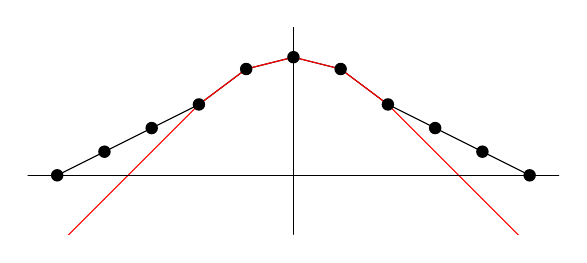
\begin{tikzpicture}[line cap=round,line join=round,>=triangle 45,scale=1.5]
      \clip(-2.25,-0.5) rectangle (2.25,1.25);
      \draw (0.4,0.9) -- (0.8,0.6);
      \draw (0.8,0.6) -- (1.2,0.4);
      \draw (1.2,0.4) -- (1.6,0.2);
      \draw (-0.4,0.9) -- (-0.8,0.6);
      \draw (-0.8,0.6) -- (-1.2,0.4);
      \draw (-1.2,0.4) -- (-1.6,0.2);
      \draw (-1.6,0.2) -- (-2,0);
      \draw (1.6,0.2) -- (2,0);
      \draw (-0.4,0.9) -- (0,1);
      \draw (0,1) -- (0.4,0.9);

      % New red curve aligning with black nodes
      \draw[red] (1.6,-.2) -- (2,-.6);
      \draw[red] (1.2,0.2) -- (1.6,-.2);
      \draw[red] (0.8,0.6) -- (1.2,0.2);
      \draw[red] (0.4,0.9) -- (0.8,0.6);
      \draw[red] (0,1) -- (0.4,0.9);
      \draw[red] (-0.4,0.9) -- (0,1);
      \draw[red] (-0.4,0.9) -- (-0.8,0.6);
      \draw[red] (-0.8,0.6) -- (-1.2,.2);
      \draw[red] (-1.2, .2) -- (-1.6,-.2);
      \draw[red] (-1.6,-.2) -- (-2,-.6);

      \begin{scriptsize}
        \fill [color=black] (-0.4,0.9) circle (1.5pt);
        \fill [color=black] (0.4,0.9) circle (1.5pt);
        \fill [color=black] (0.8,0.6) circle (1.5pt);
        \fill [color=black] (1.2,0.4) circle (1.5pt);
        \fill [color=black] (1.6,0.2) circle (1.5pt);
        \fill [color=black] (-0.8,0.6) circle (1.5pt);
        \fill [color=black] (-1.2,0.4) circle (1.5pt);
        \fill [color=black] (-1.6,0.2) circle (1.5pt);
        \fill [color=black] (-2,0) circle (1.5pt);
        \fill [color=black] (2,0) circle (1.5pt);
        \fill [color=black] (0,1) circle (1.5pt);
      \end{scriptsize}

      % Add Axes
      \draw[-] (-2.5,0) -- (2.5,0); % x-axis
      \draw[-] (0,-0.5) -- (0,1.45); % y-axis
    \end{tikzpicture}
    \caption{Iterate $u^k$(black) and obstacle $\psi$(red).}
  \end{subfigure}
  \hfill
  \begin{subfigure}[b]{.35\textwidth}
    \begin{tikzpicture}[line cap=round,line join=round,>=triangle 45,scale=1.5]
      \clip(-2.25,-0.5) rectangle (2.25,1.25);
      \draw (1.6,0) -- (2,0);
      \draw (1.2,0) -- (1.6,0);
      \draw (0.8,1) -- (1.2,0);
      \draw (0.4,1) -- (0.8,1);
      \draw (0,1) -- (0.4,1);
      \draw (-0.4,1) -- (0,1);
      \draw (-0.4,1) -- (-0.8,1);
      \draw (-0.8,1) -- (-1.2,0);
      \draw (-1.2,0) -- (-1.6,0);
      \draw (-1.6,0) -- (-2,0);

      % Add black vertices
      \begin{scriptsize}
        \fill [color=black] (1.6,0) circle (1.5pt);
        \fill [color=black] (2,0) circle (1.5pt);
        \fill [color=black] (1.2,0) circle (1.5pt);
        \fill [color=black] (0.8,1) circle (1.5pt);
        \fill [color=black] (1.2,0) circle (1.5pt);
        \fill [color=black] (0.4,1) circle (1.5pt);
        \fill [color=black] (0.8,1) circle (1.5pt);
        \fill [color=black] (0,1) circle (1.5pt);
        \fill [color=black] (0.4,1) circle (1.5pt);
        \fill [color=black] (-0.4,1) circle (1.5pt);
        \fill [color=black] (0,1) circle (1.5pt);
        \fill [color=black] (-0.4,1) circle (1.5pt);
        \fill [color=black] (-0.8,1) circle (1.5pt);
        \fill [color=black] (-1.2,0) circle (1.5pt);
        \fill [color=black] (-1.6,0) circle (1.5pt);
        \fill [color=black] (-2,0) circle (1.5pt);
      \end{scriptsize}
      
      % Add Axes
      \draw[-] (-2.5,0) -- (2.5,0); % x-axis
      \draw[-] (0,-0.5) -- (0,1.45); % y-axis
  
      % Label y=1
      \node at (-0.1,1.15) [left] {1};
      \draw[dashed] (-0.1,1) -- (0,1);
    \end{tikzpicture}
    \caption{Nodal active set indicator $s_0$.}
  \end{subfigure}
  \null\hfill
  \medskip

  \null\hfill
  \begin{subfigure}[b]{.35\textwidth}
    \centering
    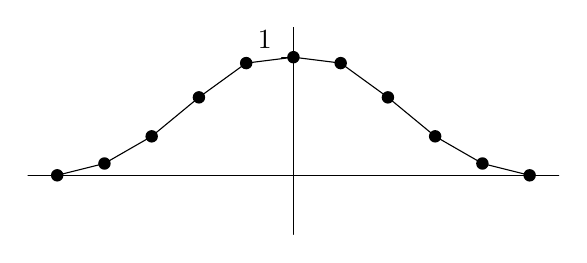
\begin{tikzpicture}[line cap=round,line join=round,>=triangle 45,scale=1.5]
      \clip(-2.25,-0.5) rectangle (2.25,1.25);
      
      % Draw the smoothed curve
      \draw (1.6, 0.1) -- (2,0);      
      \draw (1.2, 0.33) -- (1.6, 0.1);
      \draw (0.8, 0.66) -- (1.2, 0.33);
      \draw (0.4, 0.95) -- (0.8, 0.66);
      \draw (0,1) -- (0.4, 0.95);
      \draw (-0.4, 0.95) -- (0,1);
      \draw (-0.4, 0.95) -- (-0.8, 0.66);
      \draw (-0.8, 0.66) -- (-1.2, 0.33);
      \draw (-1.2, 0.33) -- (-1.6, 0.1);
      \draw (-1.6, 0.1) -- (-2,0);
  
      % Add black vertices
      \begin{scriptsize}
        \fill [color=black] (1.6, 0.1) circle (1.5pt);
        \fill [color=black] (2,0) circle (1.5pt);
        \fill [color=black] (1.2, 0.33) circle (1.5pt);
        \fill [color=black] (0.8, 0.66) circle (1.5pt);
        \fill [color=black] (0.4, 0.95) circle (1.5pt);
        \fill [color=black] (0,1) circle (1.5pt);
        \fill [color=black] (-0.4, 0.95) circle (1.5pt);
        \fill [color=black] (-0.8, 0.66) circle (1.5pt);
        \fill [color=black] (-1.2, 0.33) circle (1.5pt);
        \fill [color=black] (-1.6, 0.1) circle (1.5pt);
        \fill [color=black] (-2,0) circle (1.5pt);
      \end{scriptsize}
  
      % Add Axes
      \draw[-] (-2.5,0) -- (2.5,0); % x-axis
      \draw[-] (0,-0.5) -- (0,1.45); % y-axis
  
      % Label y=1
      \node at (-0.1,1.15) [left] {1};
      \draw[dashed] (-0.1,1) -- (0,1);
    \end{tikzpicture}
    \caption{Smoothed $s_1$.}
  \end{subfigure}
  \hfill
  \begin{subfigure}[b]{.35\textwidth}
    \centering
    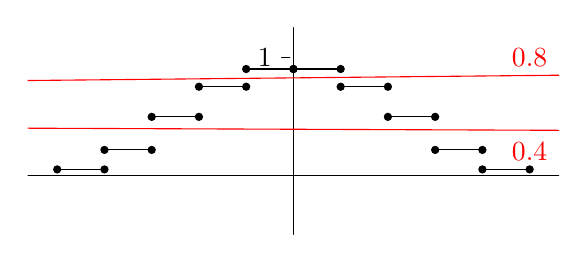
\begin{tikzpicture}[line cap=round,line join=round,>=triangle 45,scale=1.5]
      \clip(-2.25,-0.5) rectangle (2.25,1.25);

      % Draw horizontal segments at the heights of the calculated midpoints
      \draw (-2, 0.05) -- (-1.6, 0.05);
      \draw (-1.6, 0.215) -- (-1.2, 0.215);
      \draw (-1.2, 0.495) -- (-0.8, 0.495);
      \draw (-0.8, 0.75) -- (-0.4, 0.75);
      \draw (-0.4, 0.9) -- (0, 0.9);
      \draw (0, 0.9) -- (0.4, 0.9);
      \draw (0.4, 0.75) -- (0.8, 0.75);
      \draw (0.8, 0.495) -- (1.2, 0.495);
      \draw (1.2, 0.215) -- (1.6, 0.215);
      \draw (1.6, 0.05) -- (2, 0.05);

      % Add black vertices
      \begin{scriptsize}
        \fill [color=black] (-2, 0.05) circle (1pt);
        \fill [color=black] (-1.6, 0.05) circle (1pt);
        \fill [color=black] (-1.6, 0.215) circle (1pt);
        \fill [color=black] (-1.2, 0.215) circle (1pt);
        \fill [color=black] (-1.2, 0.495) circle (1pt);
        \fill [color=black] (-0.8, 0.495) circle (1pt);
        \fill [color=black] (-0.8, 0.75) circle (1pt);
        \fill [color=black] (-0.4, 0.75) circle (1pt);
        \fill [color=black] (-0.4, 0.9) circle (1pt);
        \fill [color=black] (0, 0.9) circle (1pt);
        \fill [color=black] (0, 0.9) circle (1pt);
        \fill [color=black] (0.4, 0.9) circle (1pt);
        \fill [color=black] (0.4, 0.75) circle (1pt);
        \fill [color=black] (0.8, 0.75) circle (1pt);
        \fill [color=black] (0.8, 0.495) circle (1pt);
        \fill [color=black] (1.2, 0.495) circle (1pt);
        \fill [color=black] (1.2, 0.215) circle (1pt);
        \fill [color=black] (1.6, 0.215) circle (1pt);
        \fill [color=black] (1.6, 0.05) circle (1pt);
        \fill [color=black] (2, 0.05) circle (1pt);
      \end{scriptsize}

      % Add Axes
      \draw[-] (-2.5,0) -- (2.5,0); % x-axis
      \draw[-] (0,-0.5) -- (0,1.25); % y-axis

      % Label y=1
      \node at (-0.1, 1) [left] {1};
      \draw[dashed] (-0.1, 1) -- (0, 1);

      % Add red horizontal lines at heights 0.8 and 0.4
      \draw[red] (-2.5, 0.8) -- (2.5, 0.85); % red line at y = 0.8
      \draw[red] (-2.5, 0.4) -- (2.5, 0.38);  % red line at y = 0.4
      % Label the heights of the red lines
      \node[red] at (2, 1) {0.8};
      \node[red] at (2, 0.2) {0.4};
    \end{tikzpicture}
    \caption{$interpolate(s_1,W)$. Threshold values in red.}
  \end{subfigure}
  \null\hfill
  \medskip

  \begin{subfigure}[b]{0.9\textwidth}
    \centering
    \begin{tikzpicture}[line cap=round,line join=round,>=triangle 45,scale=1.5]
      \clip(-2.5,-0.5) rectangle (2.5,1.25);
      
      \draw (1.6,0) -- (2,0);      
      \draw (1.2,0) -- (1.6,0);
      \draw (0.8,1) -- (1.2,1);
      \draw (0.4,1) -- (0.8,1);
      \draw (0,0) -- (0.4,0);
      \draw (-0.4,0) -- (0,0);
      \draw (-0.4,1) -- (-0.8,1);
      \draw (-0.8,1) -- (-1.2,1);
      \draw (-1.2,0) -- (-1.6,0);
      \draw (-1.6,0) -- (-2,0);
  
      % Add Axes
      \draw[-] (-2.5,0) -- (2.5,0); % x-axis
      \draw[-] (0,-0.5) -- (0,1.45); % y-axis
  
      % Label y=1
      \node at (-0.1, 1) [left] {1};
      \draw (-0.1, 1) -- (0, 1);
  
      % Add Nodes
      \begin{scriptsize}
      \fill [color=black] (1.6,0) circle (1.5pt);
      \fill [color=black] (2,0) circle (1.5pt);      
      \fill [color=black] (1.2,0) circle (1.5pt);
      \fill [color=black] (0.8,1) circle (1.5pt);
      \fill [color=black] (1.2,1) circle (1.5pt);
      \fill [color=black] (0.4,1) circle (1.5pt);
      \fill [color=black] (0.8,1) circle (1.5pt);
      \fill [color=black] (0,0) circle (1.5pt);
      \fill [color=black] (0.4,0) circle (1.5pt);
      \fill [color=black] (-0.4,0) circle (1.5pt);
      \fill [color=black] (0,0) circle (1.5pt);
      \fill [color=black] (-0.4,1) circle (1.5pt);
      \fill [color=black] (-0.8,1) circle (1.5pt);
      \fill [color=black] (-1.2,1) circle (1.5pt);
      \fill [color=black] (-1.2,0) circle (1.5pt);
      \fill [color=black] (-1.6,0) circle (1.5pt);
      \fill [color=black] (-2,0) circle (1.5pt);
      \end{scriptsize}
    \end{tikzpicture}
    \caption{Refinement indicator function $I$.}
  \end{subfigure}
  \vspace*{.25cm}
  \caption{Illustration of Variable Coefficient Diffusion algorithm.}
\end{figure}

Support for unstructured meshes in Firedrake comes from the DMPlex class in PETSc, as developed by \cite{LangeKnepleyGorman2015}. DMPlex is a data management object which can store the topology (connectivity of mesh entities) and geometry (coordinates) of a discretization. In the DMPlex object every mesh entity is assigned a unique index. The connectivity of a mesh is stored as a layered directed acyclic graph (DAG) in which a "covering" relation specifies the edges of the graph. For example, for a tetrahedral element in a 3d mesh, a face is covered by 3 edges and a tetrahedral cell is covered by 4 faces. Each layer represents a class of mesh entity i.e vertices, edges, etc. Below is an example of how a single tetrahedral cell is represented by DMPlex.

The DMPlex object has several methods which make querying the mesh topology and geometry simple \citep{Langeetal2016}. For example, let $p$ be an index assigned by DMPlex. Then $\emph{cone}(p)$ returns all the in-neighbors of $p$. In the example above $\emph{cone}(0) = \{11, 12, 13, 14\}$. The transitive closure of $\emph{cone}(p)$ is also available with $\emph{closure}(p)$. The dual of $\emph{cone}(p)$ is $\emph{support}(p)$ which returns all the out-neighbors of $p$. In the example above $\emph{support}(6) = \{6, 7, 10\}$. The transitive closure of $\emph{support}(p)$ is also available with $\emph{star}(p)$. 

The use of DMPlex queries is essential to our second strategy, the Unstructured Dilation Operator (UDO). We identify the set $B$ of elements that border the computed free boundary $\Gamma_{u^k}$ by interpolating a nodal active indicator function into DG0 and thresholding for values in the range (0, 1). We then use the \emph{closure} and \emph{star} methods to create vertex-to-cell and cell-to-vertex mappings. These mappings are then used to determine which elements are neighbors to the computed free boundary. We say an element neighbors another if it shares at least one vertex. The function $N(\triangle)$ returns a set of elements:
\begin{equation}
  N(\triangle) = \{\triangle_i \in T: \triangle \text{ shares at least 1 vertex with } \triangle_i\}.
\end{equation}
This process is then repeated $n$ times to create a set of elements that are within $n$ neighborhood levels of the border elements:
\begin{equation}
  N^n(\triangle) = \underbrace{N(...N(\triangle))}_{n \text{ times}}.
\end{equation}
As show in Algorithim 3, for a border element set $B$, defined below in (5.5) we use breadth-first search to construct the set $N^n(B)$ and then assemble its corresponding indicator function. This process expand the support of the DG0 indicator function in a way that resembles the "dilation" operation in image processing as seen in \citep{OpenCV} but it is applied over an unstructured mesh.

\begin{algorithm}[H]
  \caption{Unstructured Dilation Operator Element Tagging for VIs}
  \begin{algorithmic}[1]
    \Require $tol \in \mathbb{R}$, $u^k \in K, \psi \in V$, $W$ is a DGO FE space, mesh $T$.
    \Require Neighborhood Depth Parameter $n \in \mathbb{N}$.
    \State Compute the nodal active set indicator function $s$
    \begin{equation}
    s = \begin{cases}
      1 & \text{ if } u^k - \psi < tol\\
      0 & \text{ otherwise}
    \end{cases}.
    \end{equation}
  
    \State Let $s_W = interpolate(s, W)$ .
    \State Define the border element set $B$:
    \begin{equation}
    B = \{\triangle \in T: 0 < s_W(\triangle) < 1 \} .
    \end{equation}

    \State Use the \emph{closure} and \emph{star} methods to construct vertex-to-cell and cell-to-vertex mappings.

    \State Use breadth-first search to construct the set $N^n(B)$ as in (5.2) and (5.3). 
    \State Assemble the indicator function $I$ of the set $N^n(B)$. \\
    \Return $I$
  \end{algorithmic}
  \end{algorithm}

A simple example using UDO is shown.

%\inputminted{python}{short.py}

Using thresholding $u - \psi < 0.001$ to determine the active set, running this example generates the following Figure.

\begin{figure}[H]
FIXME
\caption{Mesh (left) generated from the spiral problem, with $N=2.3\times 10^3$ elements, and the approximated active set (right).}
\end{figure}


\section{Results} \label{sec:results}

FIXME discuss norm and geometric measures first

FIXME \cite{Kosub2016} \cite{JungeblutKleistMiltzow2022}

FIXME


\section{Application to determining glaciated areas} \label{sec:app}

FIXME


\section{Discussion and conclusion} \label{sec:conclusion}

FIXME \emph{Grid Sequencing + AMR targeting the free boundary} is the iterative process for how we are converging (heuristically at least) to the FB.  The bulk of vinewton iterations are coming from stabilizing the initial iterate's FB (i think) and thereafter Grid Sequencing is allowing us to make small adjustments as we refine.  A gif of the DG0 active set indicator on the sphere problem will show this, the initial iterate is completely above $\psi$ (or zero, then  projects pointwise to be feasible) then the first iteration captures the bulk of the active set, then small adjustments afterwards. On top of this the grid sequencing works best on hierarchal meshes, with metric method  the "grid sequencing" is being done through cross mesh interpolation.


%\section*{Acknowledgements}

%\section*{Notes on contributor(s)}
%An unnumbered Section, e.g.\ \verb"\section*{Notes on contributors}", may be included \emph{in the non-anonymous version} if required. A photograph may be added if requested.


\section{References}

\bibliographystyle{tfs}
\bibliography{viamr}


%Any appendices should be placed after the list of references, beginning with the command \verb"\appendix" followed by the command \verb"\section" for each appendix title, e.g.
%\appendix
%\section{This is the title of the first appendix}

\end{document}
